\section{NextDAO}
\subsection{Blockchain Collaboration}
With the emergence of the Ethereum ERC20 token that is based on the blockchain smart contract technology has become a new, fast and low-cost financing method. However, with all its benefits, the post-financing collaboration and management issues have not been well resolved which has always been one of the important development directions of blockchain and at the same time, it has shown many issues.

The DAO (Decentralized Autonomous Organization)~\cite{DAO} is an organization embodied in open and transparent computer code that is controlled by shareholders and is not affected by centralized organizations. After the release of The DAO, it was quickly hacked and millions of dollars of Ethereum was stolen which eventually led to a hard fork of the Ethereum network. Although The DAO project had defects, it has shown us many lessons to learn from and to incorporate into  follow-up work.

The Nebulas blockchain is committed to the development of blockchain collaboration and on this basis, proposes a framework based on on-chain financial collaboration entitled NextDAO. Specifically NextDAO includes: public chain collaboration, governance, decentralized finance (DeFi), etc... and is shown in detail in \ref{fig:nextdao}. NextDAO attempts to address several issues in the current blockchain collaboration model such as:

\begin{enumerate}[\hspace{1cm}(a)] 
  \item Incentives are still based on block rewards 
  \item Missing fair and positive ecosystem 
  \item Single collaboration model
\end{enumerate} 

\begin{figure}[htbp] 
  \centering 
  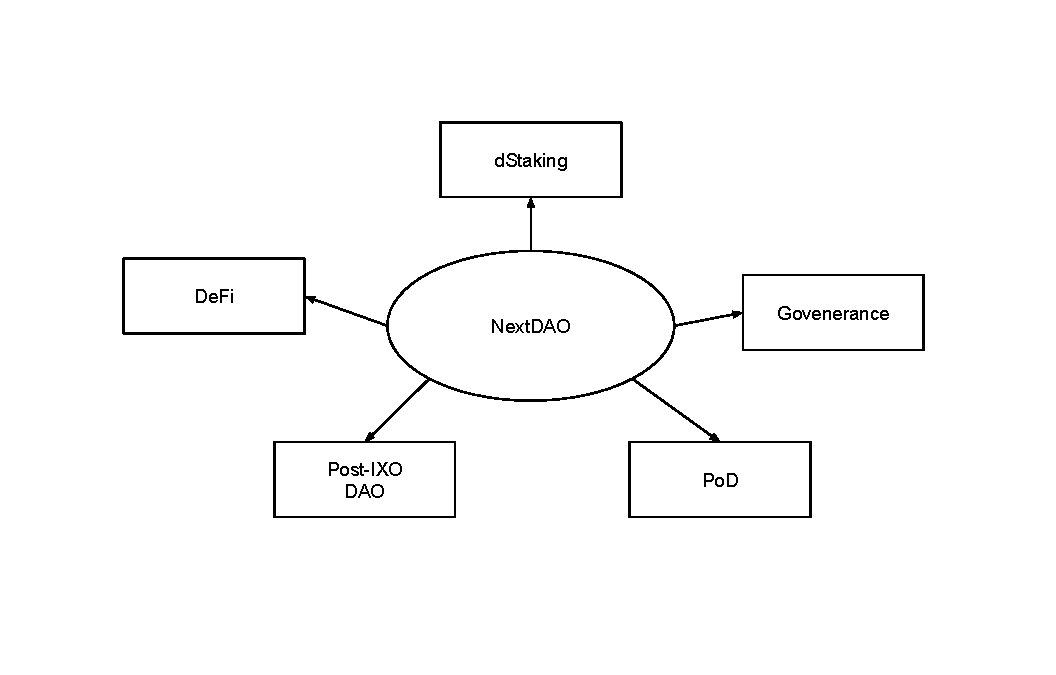
\includegraphics[width=0.5\textwidth]{../common/nextdao.pdf}
  \caption{Blockchain collaboration paradigm: NextDAO \label{fig:nextdao}} 
\end{figure} 

\subsection{Public-Chain Token Economics}
The Token Economy is embodied in an economic model that includes the generation, circulation, repurchase and incentives of issued tokens.  The general token economy exists in all corners of the blockchain world such as public chain ecosystem, decentralized applications (DApp) and so on. The typical use-case of a public chain token economy is the Ethereum ERC20 token which greatly facilitated the speed of financing and distribution leading to a stimulated economic prosperity on Ethereum as well as driving the development of the entire blockchain industry. 

Therefore, the value and innovation of the public chain is not only due to the innovation of this technology itself but also the model and commercial innovation brought by technology. The problem to be considered in the public chain token economy is the human-to-human game, and it is necessary to avoid the tragedy of the commons ~\cite{TragedyOfTheCommons} which promotes the prosperity and development of the public chain economy through positive incentives.

Most public chain projects fail in comparison when trying to compare the power of the Ethereum community. With this in mind, it's critical to design a token economy that suits it's ecosystem. A designed token economy must align with the expansion of consensus, the development of the community and a model that presents a positive ecosystem to all which will bring long-term benefits to the system. The positive development of user incentive is needed in order to promote the development of blockchain technology and its commercial expansion. The following section explores Nebulas' own vision and characteristics and presents a common on-chain based token economy paradigm based on the NextDAO framework: NAX.
